\input{../../header.tex}
\begin{document}
\section{Vorbereitung}
\label{sec:Vorbereitung}
Es wird für 10 Abstände $r$ zwischen 5 und 25\,cmdas Drehmoment auf eine Stange berechnet. 
Einmal wird die Kraft im rechten Winkel angesetzt, einmal im 45°-Winkel. \\ \noindent
\begin{figure}
    \begin{minipage}{0.39\textwidth}
    Senkrecht:\\
    $\vec M=\begin{pmatrix} 0\\F\end{pmatrix}\times
    \begin{pmatrix} r\\0\end{pmatrix}=F\cdot r\cdot\begin{pmatrix} 1\\-1\end{pmatrix}$\\
    45°-Winkel:\\
    $\vec M=\begin{pmatrix} \cos(\varphi F)\\ \sin(\varphi F)\end{pmatrix}
    \times \begin{pmatrix} r\\0 \end{pmatrix}=\\
    \begin{pmatrix} 
    \phantom{-}r\cdot F\cdot\sin(\varphi)\\ -r\cdot F\cdot\sin(\varphi)\end{pmatrix}$
    \end{minipage}
    \hfill
    \begin{minipage}{0.39\textwidth}
        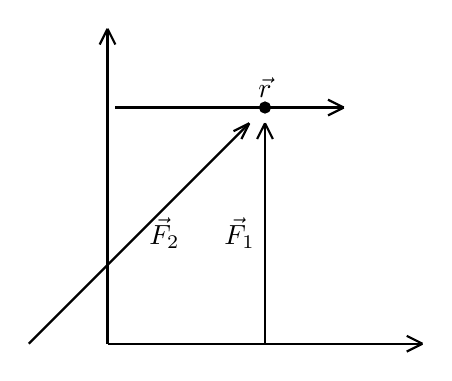
\begin{tikzpicture}
            % Koordinatensystem
            \draw[thick] (0,0) -- (0,4);
            \draw[thick] (0,0) -- (4,0);
            \draw[thick] (0,4) -- (-0.1,3.8);
            \draw[thick] (0,4) -- (0.1,3.8);
            \draw[thick] (4,0) -- (3.8,0.1);
            \draw[thick] (4,0) -- (3.8,-0.1);
            % r
            \filldraw[black] (2,3) node[above] {$\vec r$} circle (2pt);
            % Stange
            \draw[thick] (0.1,3) -- (3,3);
            \draw[thick] (3,3) -- (2.8,3.1);
            \draw[thick] (3,3) -- (2.8,2.9);
            % F_1
            \draw[thick] (2,0) -- node[left] {$\vec F_1$} (2,2.8);
            \draw[thick] (2,2.8) -- (1.9,2.6);
            \draw[thick] (2,2.8) -- (2.1,2.6);
            % F_2
            \draw[thick] (-1,0) -- node[right] {$\vec F_2$} (1.8,2.8);
            \draw[thick] (1.8,2.8) -- (1.6,2.7);
            \draw[thick] (1.8,2.8) -- (1.7,2.6);
            \end{tikzpicture}
    \end{minipage}
    \begin{minipage}{0.18\textwidth}
        \begin{tikzpicture}
        \draw[thick] (0,0) --node[left]{$\vec F_1$} (1.5,1.5);
        \draw[thick] (0,0) -- node[below] {x} (1.5,0);
        \draw[thick] (1.5,0) -- node[right] {y} (1.5,1.5);
        \draw[thick] (1,0) node[left]{\varphi} arc (0:45:1);
        \end{tikzpicture}
    \end{minipage}
\end{figure}
\end{document}